% Manuscript insertion fragment, not a standalone document.
% Requires amsmath, amssymb, and graphicx in the parent manuscript.
% Adjust the graphics path when copying into another project.
% Use figure* for a two-column paper; use figure for a single-column paper.

\paragraph{Sensitivity to partition resolution.}
We examine how the number of partitions per coordinate affects the accuracy
of the PSS entropy estimator using equicorrelated Gaussian data,
$X\sim\mathcal{N}_d(0,\Sigma)$, with $\Sigma_{ii}=1$ and
$\Sigma_{ij}=\rho=0.2$ for $i\ne j$.
We vary $d\in\{2,3,4\}$ at $n=100{,}000$ and
$n\in\{30{,}000,100{,}000,300{,}000\}$ at $d=3$.
These settings were chosen following an exploratory comparison of correlation
strengths and evaluated using new simulation seeds.
For each of the five distinct settings, we evaluate $\ell\in\{1,\ldots,8\}$
on 30 independent datasets and compute RMSE relative to the analytic Gaussian
entropy, using the same datasets for all candidate resolutions.

We compare the RMSE-minimizing resolution on this grid with a
\emph{theory-selected} resolution defined by
\begin{equation}
\begin{aligned}
\ell_{\mathrm{th}}
&=\underset{\ell\in\{1,\ldots,8\}}{\operatorname{arg\,min}}
\left\{\ell^{-2}+\sqrt{\Lambda_{n,d,\delta}}
\left(\frac{\ell^d}{n}\right)^{1/4}\right\},\\
\Lambda_{n,d,\delta}
&=2d\log(2n+1)+\log(96/\delta),\qquad\delta=0.05.
\end{aligned}
\label{eq:gaussian-theory-ell}
\end{equation}
This criterion follows the dependence on $\ell$ in the theoretical bound,
with unspecified multiplicative coefficients set to one and no fitting to
the observed errors.
Gaussian densities fall outside the theorem's bounded-support and positive
density lower-bound assumptions; this experiment therefore illustrates the
selection rule beyond those assumptions.

Figure~\ref{fig:gaussian-ell} shows that RMSE is minimized at $\ell=2$ in
all five settings. The theory-selected resolution agrees in four settings;
at $n=100{,}000$ and $d=2$, it selects $\ell=3$.
At $d=3$, the minimum RMSE decreases with increasing sample size, while finer
partitions beyond $\ell=2$ increase error in each curve.
These gridwise comparisons are descriptive and do not establish exact
finite-sample optimality.

\begin{figure*}[t]
\centering
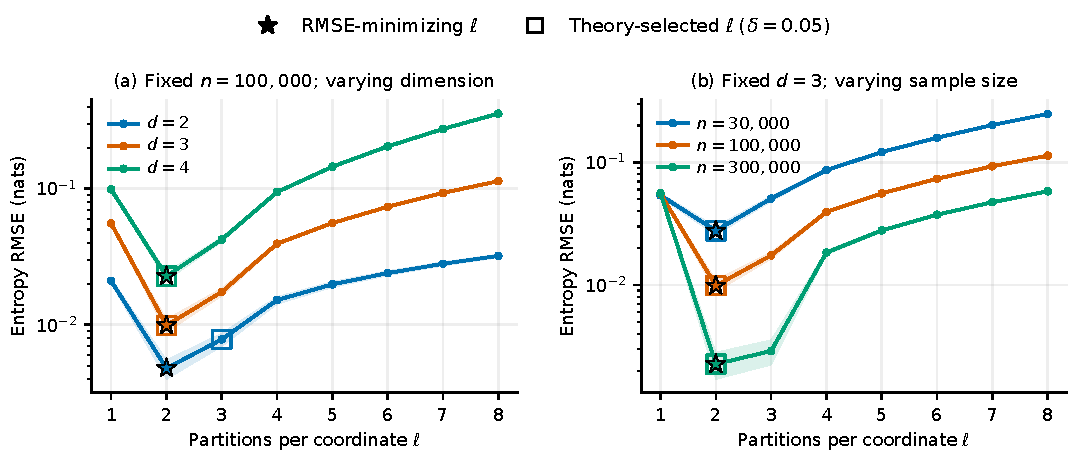
\includegraphics[width=\textwidth]{output/pdf/synthetic_gaussian_lowdim_20261006/gaussian_lowdim_ell_rmse.pdf}
\caption{Entropy-estimation RMSE versus the number of partitions per coordinate
for equicorrelated Gaussian data ($\rho=0.2$).
(a) Fixed $n=100{,}000$ and varying $d$.
(b) Fixed $d=3$ and varying $n$.
Curves use 30 independent repetitions; shading denotes pointwise 95\%
bootstrap intervals from 2,000 resamples.
Stars mark the RMSE-minimizing $\ell$ over the tested grid, using the same
repetitions as the curves. Squares mark the theory-selected $\ell$ from
Eq.~\eqref{eq:gaussian-theory-ell} at $\delta=0.05$.
The shared setting $(n,d)=(100{,}000,3)$ appears in both panels.}
\label{fig:gaussian-ell}
\end{figure*}
